\chapter{Models for the Delay}
\label{chapter4: Worm propagation}



The formalisation of the FlipIt game with delay relies on some value  \textit{d} that represents the time needed to infect a sufficient number of nodes in a network after the initial infection. This chapter provides the reader with more insight on how to calculate the value of this parameter \textit{d}.  \\

The  spreading of malware has already been extensively researched. Because of the many different types of propagation it is hard to defined a single model that can model all of them. Modelling the spread of malware depends on two key factors: the method used for the propagation and the graph where the malware will spread itself. \\
Viruses and worms are the types of malware that are the most researched. Since the spreading of viruses requires human interaction, their propagation delay is depending on (hard to predict) human behaviour. Worms on the other hand, spread without human intervention, and are their propagation is therefore easier to model. Since the purpose of this chapter is only to illustrate how a delay can be calculated, we will limit the presentation to propagation models of worms . Section \ref{methodsofpropagation} presents an overview of the most frequently used propagation methods by worms. These propagation methods will be covered by different kinds of models in section \ref{modelsforpropagation} that presents models to determine the time a worm needs to infect a sufficient number of nodes. These results can be used for the completion of parameter \textit{d}. Finally, in section \ref{eigenmatrixmethode},  we introduce an easy method to calculate the delay of the propagation of a worm.  Different kind of graphs to model a computer network are introduced. 

This chapter is based on the following papers: \cite{importantjournal}, \cite{OnWorms2005survey}, \cite{GameTheorApprCostBenefitAnalyses} and \cite{SecurelistAPT}.


\section{Methods of propagation}
\label{methodsofpropagation}

In the context of malware propagation, there exists two kinds of APT's . First, there are APT's that launch an attack on just one target node of a network. The mechanism these APT's use to propagate malware is the dropper mechanism. The dropper is the initial attack vector that compromises the single targeted node of the system. The second kind of APT's target multiple victims. These APT's also use a dropper mechanism but have an additional mechanism for self-propagation in order to propagate themselves to the multiple targeted nodes of the system. This mechanism can either be a virus propagation or a worm propagation. A virus infects one node on the network and has to wait for human interaction to spread. So the spreading speed depends on the human interaction, and modelling virus propagation therefore requires modelling human behaviour. If an APT uses a worm propagation method it will spread by itself after it has been dropped on the network. Given the additional complexity of incorporating the human factor in a spreading method and that this chapter is merely meant as illustration on calculating the delay for use in the game theoretic approach, we will limit the presentation to worm propagation models for APT's. \\

Infection by worms start with dropping the work on the network. Different dropping mechanisms can be used, whereby the initial attack can be random or targeted at a specific node. Frequently used mechanisms are USB sticks (given to a specific person or left behind for pick up by a random person), email, or malicious software through fishing or trojan horses. More important for determining our delay is the propagation strategy. Propagation is performed by determining the next nodes to spread the worm to. The following are common propagation methods: 
\begin{description}
%\item Scanning methods: A worm tries to guess (scan) the address of potential target nodes to infect. It can use distinct ways of scanning.
%% random, localized, topological or hit-list scanning.
%\begin{itemize}
\item \textbf{Selective Random scanning:} Some worms propagate by using the method of selective random targeting IP addresses. The worm selects randomly a part of the selected address space instead of scanning the whole address space. The reserved address blocks and the unassigned addresses are excluded from the address space. The rate of success for randomly chosen IP addresses is very low, but it is easy to implement. Example of such worms are `Code Red' and `Slammer'.
\item \textbf{Localized scanning:} A worm that uses localized scanning will scan for hosts in the local address space. This method is used by the `Code Red II' and `Nimda' worm.
\item \textbf{Topological scanning:} Address information stored in the victim machines are used to locate new targets. This method used by the `Morris' worm.
%\item \textbf{Hit-list scanning:} With the method of hit-list scanning, a short-list of vulnerable systems is made beforehand.  This is done to speed up the spread of worms at the initial stage. --This list consists of potentially vulnerable machines that are gathered beforehand and targeted first when the worm is released. An extreme case for the hit-list-scanning worms is a flash worm, which gathers all vulnerable machines into the list.--
\item \textbf{Sequential scanning:}
With sequential scanning, the worm will scan the IP addresses sequentially. This means that once a vulnerable host is compromised, it will look for IP addresses that are near to this host. For example, the address of the host is A, the next addresses that the worm will scan are A+1, or A-1. This method is used by the `Blaster worm'.
\item \textbf{DNS random scanning:} Another strategy is a kind of strategy in which the DNS infrastructure is used to locate a new target address. The IP address table from a DNS server is acquired from DNS records. The speed of a DNS scanning worm in the IPv6 internet is comparable to the speed of an IPv4 random scanning worm. There are some difficulties with this scanning technique. First it is difficult to obtain the whole address space from the DNS records. Secondly, the worm has to carry the database, which can slow down the propagation if the database is to big. Last, the IP addresses stored in the address table are only hosts with public domain names.
\item \textbf{Routable scanning:} The worms using routable scanning acquire target IP addresses based on the routing information in a network. Through  the BGP routing tables they can scan the routable address space. This method is three times faster than a traditional worm that uses random scanning. Examples are `Spyb0t' or `network Bluepill'. 
%--a ''routing worm'' [20]. Zou et al. designed two types of routing worms [20]. One type, based on Class-A (x.0.0.0/8) address allocations, is thus called 'ClassA routing worms.'' Such worms can reduce the scanning space to 45.3\% of the entire IPv4 address space. The other type, based on BGP routing tables, is thus called''BGP routing worms'' Such worms can reduce the scanning space to only about 28.6\% of the entire IPv4 address space.--
%\end{itemize}   

\item \textbf{Topology-based Wroms} Email and other client application worms:An email worms uses the email systems to find email addresses to propagate. Other client applications can include: Internet Relay Chat (IRC), Instant Messenger (IM), and a variety of peer-to-peer
file sharing systems, which have been used by worms to propagate in a similar way as email worms. For example, the Kak worm is a Javascript computer worm that spread itself by exploiting a bug in Outlook Express. % Another example is `GhostNet'

%Pikachu worm: The virus was mainly spread through Microsoft Outlook email attachments. The email containing the attached virus propagated through infected users by sending itself to all contacts in the user's Outlook address book. [5]
%\item \textbf{self stopping worm:} reduces speed to avoid detection. Atak worm or self stopping worm \cite{VirusChangePropSpeed}.
%\item \textbf{network sharing} `Shamoon'
%\item \textbf{shared files or spreading through SMB} (shared message block or  Common Internet File System (CIFS)) Flame
%\item \textbf{Zero-day vulnerabilities} \begin{description}
%\item Crouching Yeti is hardly a sophisticated campaign. For example, the attackers used no zero-day exploits, only exploits that are widely available on the Internet. But that did not prevent the campaign from staying under the radar for several years. \url{http://www.kaspersky.com/internet-security-center/threats/crouching-yeti-energetic-bear-malware-threat}
\end{description}

 

\section{Models for worm propagation}
\label{modelsforpropagation}
To use the models for worm propagation in our model of the FlipIt game it is sufficient to know the propagation speed of the worm and define after how many time units the network is defected. This will be equal to the \textit{d} parameter in our model.  
Stackelberg game: first move is from attacker, defender is follower. 

SI, SIR, SIS assume $\beta$ to be constant.

Continious-time model
\subsubsection{Simple Epidemic model}
%Codered paper gebruikt voor model
A Simple epidemic model is SI model. Nodes in the network can be either susceptible or infected.
Once a node is infected it will stay infected. 
The simple epidemic model is considered to be of a fixed size. The model for a fixed population is as follows:
\begin{equation}
\dfrac{d I(t)}{dt} = \beta I(t)[N-I(t)]
\end{equation} 
where I(t) is the number of infected hosts at time t; $\beta$ is the propagation rate; and N is the number of nodes in the network. In the beginning, $t=0$, I(0) hosts are infected. All the other nodes, $N - I(0)$, in the network are susceptible. 
The solution of this equation is the following logistic curve:
\begin{equation}
I = \dfrac{e^{\beta(t-T)}}{1+e^{\beta(t-T)}}
\end{equation}
where T is a time parameter representing the point of maximum increase in the
growth.\\


\begin{figure}[hbtp]
\centering
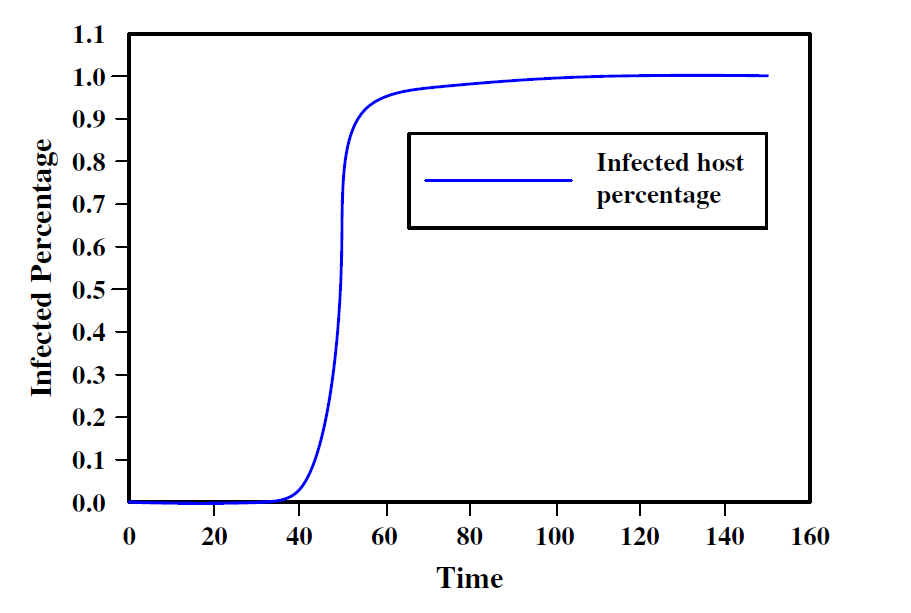
\includegraphics[scale=0.5]{Images/SEMmodel.png}
\caption{Simple Epidemic Model. The x-coordinate is the propagation time and the y-coordinate is the infected percentage of the whole network. Original image from \cite{OnWorms2005survey}}
\label{SEMmodel}
\end{figure}

Figuur \ref{SEMmodel} laat het SEM model zien.
This Simple epidemic model has been used in various papers \cite{OwnInternetSI} \cite{CodeRed} to model random scanning worm such as Code Red and Slammer. \\
For our paper we have to approximate the propagation speed en Infect gelijkstellen aan het aantal genoeg nodes die geinfecteerd moeten zijn door de APT om de controle te hebben. Dan weten we hoelang het duurt. In het begin zullen er ook geen geinfecteerde hosts zijn, dus de vergelijking kan opgelost worden.\\
Er wordt geen rekening gehouden met de topology ? nog uitzoeken.
\subsubsection{Kermack-Mckendrick model: SIR}
In the Kermack-Mckendrick model, also known as SIR model, nodes can have three states: susceptible, infected or removed. Once a node of the network has been recovered from a worm, the node will stay in the removed mode and never becomes infected again. These nodes are not able to infect other nodes and can no longer be infected. \\
Let I(t) be the number of infectious hosts at time \textit{t}, R(t) be the number of removed hosts at time \textit{t} and J(t) is the number of infected hosts by time \textit{i}, regardless the fact that a node can be in a removed state.
\begin{equation}
J(t) = I(t) + R(t).
\end{equation} 
The Kermack-McKendrick model can be represented as follows:
\begin{equation}
\begin{Bmatrix} \dfrac{d J(t)}{dt} = \beta J(t) \big[N- J(t) \\
\dfrac{d R(t)}{dt} = \gamma I(t) \\
J(t) = I(t) + R(t) = N - S(t)
 \end{Bmatrix}
\end{equation}
Parameter $\beta$ is again the rate of infection and $\gamma$ is the rate of removal of infected hosts. S(T) is the number of susceptible hosts at time t.
\begin{figure}[hbtp]
\centering
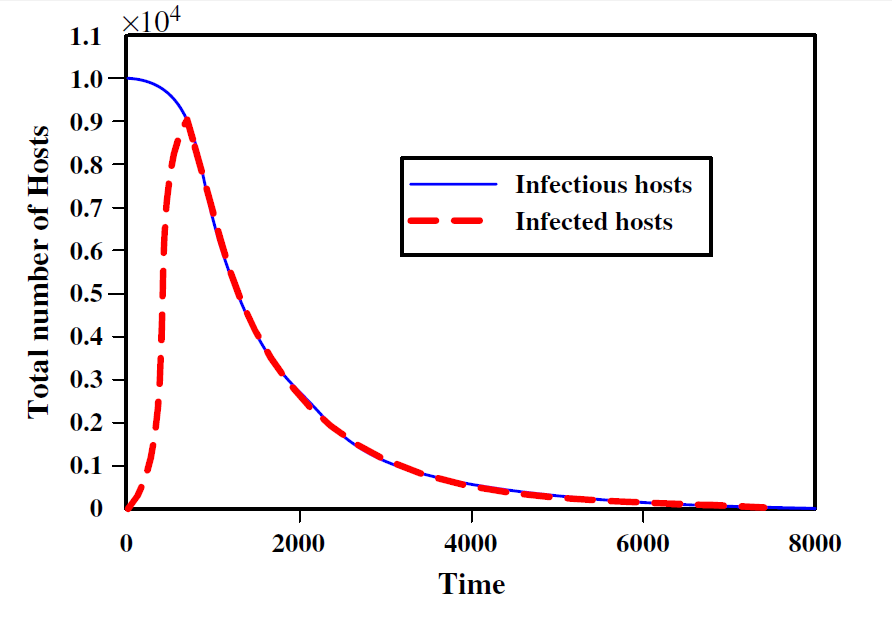
\includegraphics[scale=0.5]{Images/KMmodel.png}
\caption{KM Model. The x-coordinate is the propagation time and the y-coordinate is the infected percentage of the whole network. Original image from \cite{OnWorms2005survey}. $N=10000, \beta = 1/10000000$.}
\label{KMmodel}
\end{figure}

%codered%
--Define $\rho = \gamma/\beta$ to be the relative removal rate [3]. One
interesting result coming out of this model is
dI(t)
dt > 0 if and only if S(t) > p. (6)
Since there is no new susceptible host to be generated,
the number of susceptible hosts S(t) is a monotonically decreasing
function of time t. If S(t0) < p, then S(t) < p and
dI(t)/dt < 0 for all future time t>t0. In other words, if the
initial number of susceptible hosts is smaller than some critical
value, S(0) < p, there will be no epidemic and outbreak
[15].
The Kermack-Mckendrick model improves the classical
simple epidemic model by considering that some infectious
hosts either recover or die after some time. However, this
model is still not suitable for modeling Internet worm propagation.
First, in the Internet, cleaning, patching, and filtering
countermeasures against worms will remove both susceptible
hosts and infectious hosts from circulation, but KermackMckendrick
model only accounts for the removal of infectious
hosts. Second, this model assumes the infection rate
to be constant, which isn't true for a rampantly spreading
Internet worm such as the Code Red worm--
\subsubsection*{SIS}


\subsubsection{Two-Factor model}
%distributed worm simulation
--Zou et
al. [15] present a ''two-factor'' model that extends SIR
epidemiological model to capture the effects of human
countermeasures and the congestion due to the worm
spread. Shen et al. [16] provide a discrete-time worm
model that considers patching and cleaning effect and can
model worms with local scanning techniques. All these
approaches abstract specifics of the Internet topology,
change in the size of vulnerable population as the worm
spreads, and the effect of the individual host and network
defenses (except for patching, in case of [16]) on the
spread--
\subsubsection*{self disciplinary worms}
Model for self disciplinary worms and counter measures ... []

Popular mechanism that worms use to detect vulnerable targets by random IP scanning probing. Feasible due to use 32-bit addresses. 128-bit addresses life harder for worms, except the ones that use email systems to propagate. two new strategies: uniformly distributed random number generator to select new target. :spread locally, by biasing the search space towards addresses within the same subnet or network.  
The second strategy is almost the same as what email virusses would get. For this reason we work an example out .. 



A method to calculate the propagation of the virus in an easy way. Google page ranking algorithm. 

\todo{toch eigen methode introduceren}




\section{methode met matrixen}
\label{eigenmatrixmethode}

All of the above models for modelling the mechanism of the spreading of a worm depend on the kind of topology of the network. In this chapter we propose a method to calculate the spread of the worm in way where the topology of the network is easily integrated. The method will give an approximation of how fast a worm can infect a network. The method is based on the method for Google Page Ranking \todo{ref} []. 
or some of the spreading methods, the graph of the network matters. It is important to have the right topology for the right method. Email worms need a topology that represent a social network, BGP routing worms need a topology on network level. 
--iets zeggen dat het ook belangrijk is voor de defender om zijn netwerk zo aan te passen dat het virus moeilijker kan verspreiden. Network segregation mss aanhalen ?--

\begin{description}
\item Power law
\item Small world topology
\item random graph
\item ..
\end{description}

%The usefulness of this method is that it is graph model independent. The topology of the network has to be in the form of a square matrix. Each connection is determined by the entries on the matrix. 
%$N_{0}$ denotes the initially infected resources at the beginning of the virus propagation. 
%$P_{x}(R_{n},t|R_{0},r,t_{0})$ denotes the chance that resource $R_{n}$ is infected at time $t$ after dropping virus number x on to resource $R_{0}$ at $t_{0}$ with rate $r$. \\

%$S(R_{n},R_{0})$ denotes the shortest path from the infected resource $R_{0}$ to resource $R_{n}$. It gives back a value with the distance measured with how many resources are in between including the end resource. \\

%So the chance that a resource is infected after time t is the chance that the resource is infected by all the previous infections and that the defender has not flipped the resource.

The computer network can be modelled by an undirected Graph $G = < V, E> $ where $|V|$ denotes the number of resources in the network and $|E|$ the number of connections. We can convert this to an adjacency matrix which represents which vertices of the graph are neighbours of other vertices. \\
The graph is represented as a $|V| \times |V|$ matrix with for every entry $a_{ij}$ a 1 as value if there is a connection between node $V_{i}$ and $V_{j}$ and 0 otherwise, and with 0's for every $a_{ii}$. Because the graph is undirected we have a symmetric matrix.  \\ 

Adjacency matrices have many interesting applications, amongst which calculating the paths between vertices:
\textit{``If \textit{A} is the adjacency matrix of the directed or undirected graph \textit{G}, then the matrix $A^{n}$ (i.e., the matrix product of \textit{n} copies of \textit{A}) has an interesting interpretation: the entry in row \textit{i} and column \textit{j} gives the number of (directed or undirected) walks of length \textit{n} from vertex \textit{i} to vertex \textit{j}. If \textit{n} is the smallest nonnegative integer, such that for all i ,j , the (i,j)-entry of $A^{n} > 0$, then n is the distance between vertex i and vertex \textit{j}.''}  source: \cite{wikimatrix} .\\


%%% Local Variables: 
%%% mode: latex
%%% TeX-master: "thesis"
%%% End: 
\begin{figure}
\centering
\begin{tikzpicture}[->,>=stealth',shorten >=1pt,auto,node distance=2.8cm,
                    semithick]
  \tikzstyle{every state}=[fill=blue,draw=none,text=white]

  \node[initial,state] (A)                    {$N_1$};
  \node[state]         (B) [above right of=A] {$N_2$};
  \node[state]         (D) [below right of=A] {$N_3$};
  \node[state]         (C) [below right of=B] {$N_4$};
  \node[state]         (E) [below right of=C] {$N_5$};
  \node[state]		   (F) [above right of=C] {$N_6$};

  \path (A) edge              node {} (B)
            edge              node {} (D)
        (B) edge              node {} (A)
        	edge			  node {} (C)
        (C) edge              node {} (B)
            edge 			  node {} (D)
            edge			  node {} (E)
            edge			  node {} (F)
        (D) edge 			  node {} (C)
            edge              node {} (A)
        (E) edge 			  node {} (C)
    	(F)	edge			  node {} (C);
\end{tikzpicture}
\caption{Network with 6 nodes. The arrows represent the connections between the nodes. The start point is were the worm has been dropped, here node 1.}
\label{netwerkfiguur}
\end{figure}

%\[
%\begin{bmatrix}
%    x_{11}       & x_{12} & x_{13} & \dots & x_{1n} \\
%    x_{21}       & x_{22} & x_{23} & \dots & x_{2n} \\
%    \hdotsfor{5} \\
%    x_{d1}       & x_{d2} & x_{d3} & \dots & x_{dn}
%\end{bmatrix}
%=
%\begin{bmatrix}
%    x_{11} & x_{12} & x_{13} & \dots  & x_{1n} \\
%    x_{21} & x_{22} & x_{23} & \dots  & x_{2n} \\
%    \vdots & \vdots & \vdots & \ddots & \vdots \\
%    x_{d1} & x_{d2} & x_{d3} & \dots  & x_{dn}
%\end{bmatrix}
%\] 
Assuming a network like in figure \ref{netwerkfiguur}, the corresponding adjacency matrix is the  matrix $[A]$: \\


$
\bordermatrix{
         & N_1		& N_2	& N_3	& N_4 	& N_5	&N_6     \cr
    N_1   & 0		& 1		& 1		& 0		& 0		& 0	     \cr
    N_2   & 1		& 0		& 0		& 1		& 0		& 0	     \cr
    N_3   & 1		& 0		& 0		& 1		& 0		& 0	     \cr
    N_4   & 0		& 1		& 1		& 0		& 1		& 1	     \cr
	N_5   & 0		& 0		& 0		& 1		& 0		& 0	     \cr
	N_6   & 0		& 0		& 0		& 1		& 0		& 0	     \cr
}$
\\

In matrix $A \times A = A^{2}$, each entry represents the number of 2 step paths from $N_{i}$ to $N_{j}$: We denote this matrix as matrix \textit{[B]}\\


$
\bordermatrix{
         & N_1		& N_2	& N_3	& N_4 	& N_5	&N_6     \cr
    N_1   & 2		& 0		& 0		& 2		& 0		& 0	     \cr
    N_2   & 0		& 2		& 2		& 0		& 1		& 1	     \cr
    N_3   & 0		& 2		& 2		& 0		& 1		& 1	     \cr
    N_4   & 2		& 0		& 0		& 4		& 0		& 0	     \cr
	N_5   & 0		& 1		& 1		& 0		& 1		& 1	     \cr
	N_6   & 0		& 1		& 1		& 0		& 1		& 1	     \cr
}$
\\

Likewise, in matrix $A^{2} \times A = A^{3}$ each entry represents the number of paths with 3 steps from $N_{i}$ to $N_{j}$: We denote this matrix as matrix \textit{[C]}\\


$
\bordermatrix{
         & N_1		& N_2	& N_3	& N_4 	& N_5	&N_6     \cr
    N_1   & 0		& 4		& 4		& 0		& 2		& 2	     \cr
    N_2   & 4		& 0		& 0		& 6		& 0		& 0	     \cr
    N_3   & 4		& 0		& 0		& 6		& 0		& 0	     \cr
    N_4   & 0		& 6		& 6		& 0		& 4		& 4	     \cr
	N_5   & 2		& 0		& 0		& 4		& 0		& 0	     \cr
	N_6   & 2		& 0		& 0		& 4		& 0		& 0	     \cr
}$ 


~~\\
So, in $A^{N}$ every $a_{ij}$ entry gives the number of paths with N steps from $N_{i}$ to $N_{j}$.\\

Using this knowledge we can calculate in how many steps a node is infected: \\
The infection vector or start vector $I_{0}$ of lenght $|V|$ indicates which node is infected and which not. Multiplying the infection vector with $A$ results in a vector $I_{1}$, which represents which nodes are infected after 1 step. Multiplying the start vector $I_{0}$ with $A^{N}$ calculates which nodes are infected in \textit{N} steps: each non zero entry represents an node infected after \textit{N} steps. \\
In the context of the FlipIt game, it is safe to assume that once a node is infected, it stays infected until the defender Flips the node. This means that after d steps, it is assumed that all nodes that could be reached in less than \textit{d} steps from the node where the worm was dropped, are infected. In order to know how many nodes are infected after (for example) at most 3 steps, we have to consider nodes that are infected initially (step 1), or after 2 steps, or after 3 steps.  Calculating the sum of the three matrices $(A + A^{2} + A^{3}) $ results in a matrix that indicates for each node, the number of paths of length 1, 2 or 3 from \textit{i} to \textit{ j}. Multiplying the start vector with this matrix, results in a vector that indicates which nodes will be infected in at most 3 steps . This technique can be applied to calculate the state of the network after any number of steps. \\

Determining the length of the delay boils down to determining which configuration of infected nodes is considered as corresponding to the attacker having flipped the resource. It may be that all nodes need to be flipped, a sufficient amount of nodes, or a (set of) particular nodes.\\

--Hier nog een beetje verder uitschrijven hoe je exact de d dan moet bepalen, gegeven dat je niet weet in welke knoop het virus gedropt wordt-- \\


%What do we need for an algorithm
%\begin{description}
%\item Graph network $G = < V, E>$
%\item Graph matrix $[A]$ which is $|V| \times |V| $
%\item Attack vector $[X]$ which is $1 \times |V|$
%\item cummulative matrix $[M]$ which is $|V| \times |V|$
%\item state matrix $[T]$  which is $|V| \times |V|$
%\item Reset vector $[R]$
%\item duration \textit{d}
%\item time \textit{n}
%\item rate $\delta _{0}$ of defender and $\delta _{1}$ of attacker
%\end{description}
%
%
%
%Initialisation algorithm:
%
%
%\begin{verbatim}
%initialisatie
%	d=0
%	A=basismatrix
%	M=A^{0}
%	n=0
%	\delta_{0}
%	\delta_{1}
%	X
%	R
%	controller = defender
%	
%	
%
%	Algorithm
%	n:= n + 1;
%	Check who is in control? ( through modulo )
%	if ( defender & controller=defender)
%				d:= d + 1;
%	
%	if ( defender & controller=attacker )
%				G = X \times R  (flippen ten voordele van defender)
%				d = 0
%				controller = defender
%				
%	if ( attacker & controller=defender )
%				controller=attacker
%				..
%				
%	if ( attacker & contoller=attacker )
%				d:= d + 1
%				M = M x A
%				T = T + M
%				G = X x T
%				
%		
%\end{verbatim}


%\end{document}
